\chapter{基于混合纠删码的数据修复技术研究}

\section{引言}
数据恢复一般有两种技术:重构(reconstruction)和退化读(degraded read)。
重构是指数据已经在存储设备中丢失,在实际的数据修复后
将其存储到新的设备中。 退化读指的是在应对暂时性
故障时,恢复操作读取的数据不必写入到设备中。 研
究一般集中在降低数据修复时所需要读取与传输的数
据量上,缓解高退化读的延迟问题。

在传统的存储系统中大多只采用一种纠删码进行
数据的处理和存储,这种方式一般先将文件分割成固
定大小的数据块,再将这些数据块每$k$
个作为一组,
每组独立进行编码操作生成$n$
个块,其中$n$
个块的集合
称为一个条带(Stripe),然而这种方式难以在保持低
存储空间消耗的情况下降低退化读的延迟时间。最
近,一些系统开始采用多副本技术与纠删码混合或者
混合纠删码的方式来进行数据的存储\cite{ma2013ensemble,friedman2014replicated,xia2015tale}。
\citet{friedman2014replicated,xia2015tale}设计了一种融合了多副本技术和纠删码技术存储系统。
而在\citet{xia2015tale}提出的HACFS中,将从属于同一码种(product code和LRC)但不同参数的纠删码部署到系统中,分别处理冷数据和热数据。
然而,由于选取了同一码族的编码,该码族的既定缺陷将难以避免。
如采用 product code(PC)时,其编码特性使得这一策略无论如何最多允许丢失三个数据块;
而不论是采用PC还是LRC,其存储冷数据时所采用编码均不是MDS的,在存储开销方面存在缺陷。
为了改进此问题,\citet{wang2020adaptive}尝试选取来自不同码族的两种编码,即LRC和HH(Hitchhiker)码来组成混合存储策略。
目的是为了降低系统总体的退化读延迟,且对于热数据采用低恢复延迟的编码,冷数据采取保证MDS特性的编码。然后问题在于,虽然
LRC\&HH码的方案可以通过downcode和upcode的方式将数据存储从两种编码之间进行切换,但却没有良好的自适应负载,亦即
没有针对数据的I/O特点针对性地提出各种负载场景下数据的动态切换方案。

本文在前文预先修复的单一纠删码的基础上,进一步推进了纠删码修复技术的应用。在\citet{wang2020adaptive}工作的基础上,
提出了一种可感知数据热度的负载动态自适应的混合纠删码(LRC\&HH)数据修复方案。
旨在根据真实储存系统数据修复场景中的数据I/O的特点,以及数据访问和故障事件的时空局部性,提出更加符合相应情况的混合纠删码
修复方案,从而对于计算开销型修复任务降低其开销和存储成本,对读取密集型和频繁重建型修复任务降低其工作负载,并加速系统的
修复速度和减少重建时间。

\section{编码策略选择}
为了选择出一对合适的编码策略来适应性地调整数据存储和恢复性能,本文总结了以下要求。
\begin{enumerate}
	\item 两种编码策略应该有类似的布局,更加方便且低成本地建立它们之间的转换;
	\item 两种编码策略应具有较高的灵活性,以支持任意数量的存储节点,并且可以适用于负载平衡的任务要求;
	\item 两种编码策略在数据存储和数据修复任务中分别发挥不同的作用,实现功能上的互补。
\end{enumerate}

\subsection{局部修复码(LRC)}

LRC在传统RS编码的基础上,引入局部分组的思想,将编码块划分成多个小分组,分组内部生成局部校验块进行容错保护。
数据修复不再完全依赖于全局校验组,优先使用局部分组内的数据进行重建,从而通过减少参与节点的数量,降低了修复过程中的网络传输开销和磁盘读取开销。
在LRC中,$m$个冗余块被细分为全局冗余块及局部冗余块,
两者的块数是LRC中的重要参数。记一个LRC编码中全局冗余块的块数为$g$,
局部冗余块的块数为$l$,就有$m = g + l$;这样的一个LRC被记为LRC$(k,l,g)$。在进行
LRC$(k,l,g)$的编码操作时,首先将$k$个数据块通过一个RS$(k,g)$
码编码得到$g$个全局冗余块,
之后将$k$个数据块(相对)平均地分为$l$个组,
每一组将对应一个局部冗余块。 
在每一组中,局部冗余块将通过这一组中的数据块直接进行异或运算得到。

局部冗余块的设置减少了恢复数据时需要访问的节点数。 
当一个数据块需要恢复时,只需要获取它所在分组对应的局部冗余块及分组中其余的数据块,
便可以对它们进行异或运算得出恢复结果。一个LRC$(k,l,g)$恢复一个数据块需要另外$k/l$块,
而对应的一个RS$(k,g)$码则需要$k$块,是前者的$l$倍。如图~\ref{fig:4.1}所示,是LRC$(6,2,2)$的具体组合方式,
其中$p_x$和$p_y$是两个全局冗余块,而两个数据块被平均地分为了三组$(x_1,x_2)$,$(y_1,y_2)$,$(z_1,z_2)$,它们
分别对应的局部冗余块为$p_{xy}$和$p_{yz}$。当$x_1$需要被修复时,只需要获取$x_2,y_1$和$p_{xy}$即可。


\begin{figure}[htbp]
	\centering
	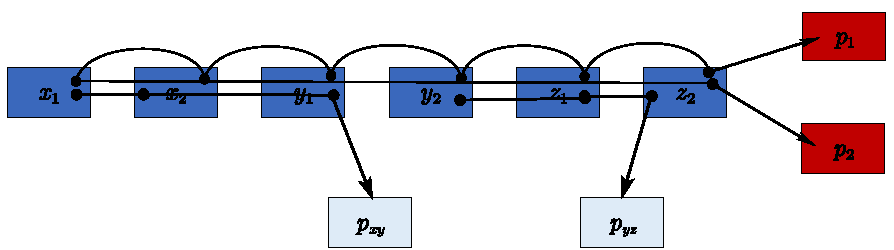
\includegraphics [scale=0.7]{figures/4.1.pdf}
	\caption{LRC(6,2,2)的组成}
	\label{fig:4.1}
\end{figure}

\subsection{Hitchhiker(HH)码}

在一个HH$(k,m)$码中,每个条带被分为两个子条带,分别为$a={a_i}$和$b={b_i}$,
且其中有$k$个数据块和$m$个校验块。在编码计算中,同一个子条带中的数据首先会被编码成RS$(k,m)$,从而得到校验块
$f_i(a)$和$f_i(b)(1\leqslant i\leqslant m)$。然后,将子条带$a$中的$k$个数据块平均地分为$(m-1)$组,每个组
$G_i$对应子条带$b$中的校验块$b_{k+i+1}$,最后将$G_i$和$f_{i+1}(a)$中的数据块进行XOR计算。

在丢失一个数据块时,
设其在$a$中的子数据块在上述分组中对应$g_t(a)$。
首先通过子条带$b$中可用的另外$(k-1)$个数据块以及$f_1(b)$,可以恢复得到丢
失的在$b$中的子数据块,进而可以求出$f_{(t-k)}(b)$。而$a$中子数据块
则可以通过上述分组中同一组内其余的$a$中子数据块,子条带$b$的第$t$个子块,
以及刚刚求出的$f_{(t-k)}(b)$进行异或运算得到。 
这样,要恢复一个数据块,需要读取的子数据块数为$k+\frac{k}{m-1}=\frac{km}{m-1}$,
折合为$\frac{km}{2(m-1)}$块,相比于RS码需要$k$块,在$m \geqslant 3$时均有较为明显的减少。

如图~\ref{fig:4.2}所示,展示的是HH$(12,4)$组成,如果想修复$a_1$和$b_1$,首先需要读取$b_2$到$b_{13}$总共12个数据块。
这12个数据块足以恢复出$b_1$,然后可以计算出$b_{14}$对应的RS校验块$f_2(b)$。
最后,再读取$a_2$到$a_4$和$b_{14}$,计算出$a_1=a_2\oplus a_3 \oplus a_4 \oplus b_{14} \oplus f_2(b)$。
总共需要读取16个数据块,相比RS码少读了8个数据块。

\begin{figure}[htbp]
	\centering
	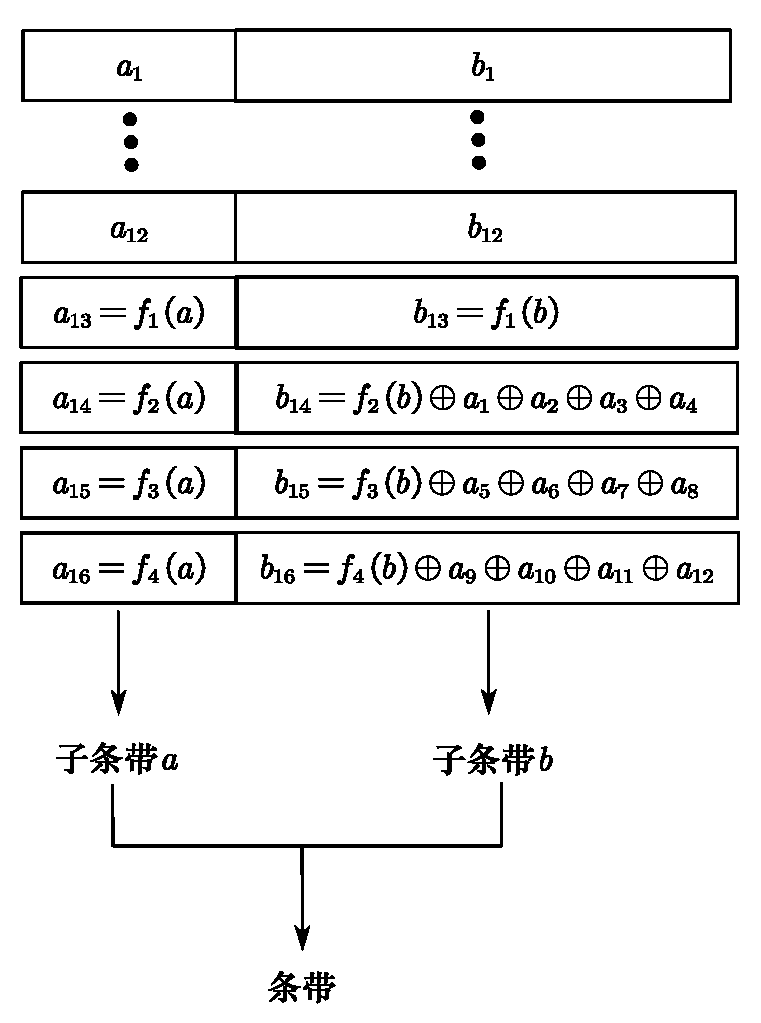
\includegraphics [scale=0.5]{figures/4.2.pdf}
	\caption{HH$(12,4)$码组成}
	\label{fig:4.2}
\end{figure}

\section{负载自适应策略}
\label{Section:4.3}

受\citet{qiu2020ec}工作的启发,针对实际存储系统数据I/O的特点,本文静态地将数据分为六类(如表~\ref{table:4-1}所示),其中风险指的是因数据丢失而产生对系统风险的影响。
1)低风险的冷数据;2)高风险的冷数据;3)低风险的写入密集型数据;
4)高风险的写入密集型数据;5)低风险的读取密集型数据;6)高风险的读取密集型数据。
其中,读取密集型和写入密集型数据都属于热数据,而读写平衡的系统应用可以属于写入密集型或读取密集型。
一般来说在低风险环境下,这种应用更可能是写入密集型的,因为整体性能主要受写入操作的影响。
然后可以确定为其分配何种编码,并为数据的动态I/O提供自适应方法。

\begin{table}[htbp]
	% \setlength{\tabcolsep}{2.9pt}
	\centering
	\caption{不同系统负载情况下的编码分配方案}
	\begin{tabular}{cccc}
		\toprule
        \multicolumn{2}{c}{\multirow{2}*{编码策略}}          & \multicolumn{2}{c}{修复负载} \\
         &                                      & 高风险             & 低风险    \\[2pt]
        \hline
		\\[-15pt]
        \multirow{3}{*}{系统负载} & 写入密集型 & LRC或HH & Hitchhiker  \\
                                                & 读取密集型 & LRC & Hitchhiker  \\
                                                & 冷数据 & Hitchhiker & Hitchhiker  \\
		\midrule
	\end{tabular}
	\label{table:4-1}
\end{table}



\subsection{编码分配规则}
\label{subsection:4.1}
为了让不同的数据和读写任务工作负载情况匹配上适当的编码方案,
显然可以得到如表~\ref{table:4-1}中总结了编码分配策略。直观地说,冷数据或低风险数据可以选择存储开销较低的HH码,
这样可以保持较高的存储效率,以及良好的系统可靠性。特别是对于写入密集型I/O的任务,
而对于具有高故障风险且以读为主的数据,LRC码可以节省大量的重建带宽,并对I/O速度造成更少的负面影响。
然而,对于高风险的写入密集型数据,难以选择一个合适的编码策略,因需要在系统的读取性能和修复I/O之间进行平衡,
从而确定合适的编码来最大化系统的整体性能。为了解决这个问题,本文进行了如下计算,最终结果呈现在表~\ref{table:4-2}。

\textbf{读写负载模式}。首先确定RS$(k,r)$在单个数据块上的计算性能消耗$RWCost_{compute}^{RS}$,
磁盘I/O消耗$RWCost_{I/O}^{RS}$,传输消耗$RWCost_{transmission}^{RS}$。
设系统读写调度的写入速度为$v_w$,读取速度为$v_r$,一个数据块大小为$\gamma$,那么对于
RS$(k,r)$而言,其编码过程中的GF运算次数等价于运算复杂度即$k \times r$,而对于读写交叉的任务而言其所占据的比例为$\frac{v_w}{v_w+v_r}$,
故在读写负载模式中RS$(k,r)$的计算性能消耗$RWCost_{compute}^{RS}$为:
\begin{equation}
	\label{eq:4-1}
	RWCost_{compute}^{RS} = \frac{v_w}{v_w+v_r} \gamma kr
\end{equation}
这里令$\frac{v_w}{v_r}$为$\beta$,则式~\ref{eq:4-1}可改写为:

\begin{equation}
	\label{eq:4-2}
	RWCost_{compute}^{RS} = \frac{\beta}{1+\beta} \gamma kr
\end{equation}

设磁盘一次I/O可传输的字节数为$\phi$,则可得到读写负载模式中RS$(k,r)$的磁盘I/O消耗$RWCost_{I/O}^{RS}$为:
\begin{equation}
	\label{eq:4-3}
	RWCost_{I/O}^{RS} = \frac{\gamma}{\phi}
\end{equation}

对于传输消耗$RWCost_{transmission}^{RS}$,分为读取传输和写入传输,其中读取任务的传输消耗为$\frac{v_r}{v_r+v_w}$,
写入任务的传输消耗为$\frac{v_w\frac{r+k}{k}}{v_r+v_w}$。那么读写负载模式中RS$(k,r)$的
传输消耗$RWCost_{transmission}^{RS}$为:

\begin{equation}
	\begin{aligned}
	\label{eq:4-4}
	RWCost_{transmission}^{RS} & = \frac{v_r}{v_r+v_w} + \frac{v_w\frac{r+k}{k}}{v_r+v_w} \\
	                    & = \frac{1}{1+\beta} + \frac{\beta}{1+\beta} \cdot \frac{r+k}{k} \\
						& = \frac{\beta(r+k)+k}{k(1 + \beta)} \\
						& = 1 + \frac{\beta}{1 + \beta} \cdot \frac{r}{k}
	\end{aligned}
\end{equation}

由于LRC$(k,l,g)$恢复一个数据块需要另外$k/l$块,
而对应的一个RS$(k,g)$码则需要$k$块,是前者的$l$倍。
故将其分别代入式~\ref{eq:4-2},式~\ref{eq:4-3},式~\ref{eq:4-4},则可以得到读写负载模式中LRC$(k,l,g)$的
计算性能消耗$RWCost_{compute}^{LRC}$,
磁盘I/O消耗$RWCost_{I/O}^{LRC}$,传输消耗$RWCost_{transmission}^{LRC}$分别为:
\begin{equation}
	\label{eq:4-5}
	RWCost_{compute}^{LRC} = \frac{\beta}{l(1+\beta)} \gamma kr
\end{equation}
\begin{equation}
	\label{eq:4-6}
	RWCost_{I/O}^{LRC} = \frac{\gamma}{\phi}
\end{equation}
\begin{equation}
	\label{eq:4-7}
	RWCost_{transmission}^{LRC} = 1 + \frac{\beta}{k(1 + \beta)} \cdot rl
\end{equation}

同样,对于HH码,其需要读取$\frac{km}{2(m-1)}$块数据进行处理,分别将其代入式~\ref{eq:4-2},式~\ref{eq:4-3},式~\ref{eq:4-4},
则可以得到读写负载模式中HH$(k,m)$的
计算性能消耗$RWCost_{compute}^{HH}$,
磁盘I/O消耗$RWCost_{I/O}^{HH}$,传输消耗$RWCost_{transmission}^{HH}$分别为:
\begin{equation}
	\label{eq:4-8}
	RWCost_{compute}^{HH} = \frac{\gamma \beta kmr}{2(1+\beta)(m-1)}
\end{equation}
\begin{equation}
	\label{eq:4-9}
	RWCost_{I/O}^{HH} = \frac{\gamma}{\phi}
\end{equation}
\begin{equation}
	\label{eq:4-10}
	RWCost_{transmission}^{HH} = 1 + \frac{\beta}{1 + \beta} \cdot \frac{2r(m-1)}{km}
\end{equation}


\textbf{修复负载模式}。与读写模式相同,首先确定RS$(k,r)$在修复负载模式下单个数据块上的计算性能消耗$RecoverCost_{compute}^{RS}$,
磁盘I/O消耗$RecoverCost_{I/O}^{RS}$,传输消耗$RecoverCost_{transmission}^{RS}$。
因在修复过程中需要传输$k$个数据块和$(r+k)\times r \times r$\cite{qiu2020ec}次运算,故修复负载模式下的RS$(n,k)$的计算性能消耗$RecoverCost_{compute}^{RS}$为:
\begin{equation}
	\label{eq:4-11}
	RecoverCost_{compute}^{RS} = (r+k)r^2+\gamma k
\end{equation}
同样可得,修复负载模式下的RS$(n,k)$的磁盘I/O消耗$RecoverCost_{I/O}^{RS}$为:

\begin{equation}
	\label{eq:4-12}
	RecoverCost_{I/O}^{RS} = \frac{\gamma}{\phi}
\end{equation}
显然,修复时需要传输$k$个数据块,则传输消耗$RecoverCost_{transmission}^{RS}$为:
\begin{equation}
	\label{eq:4-13}
	RecoverCost_{transmission}^{RS} = k
\end{equation}

同理,分别将LRC码的$\frac{k}{l}$和HH码的$\frac{km}{2(m-1)}$代入到式~\ref{eq:4-11},~\ref{eq:4-12},~\ref{eq:4-13},可得
修复负载模式中LRC$(k,l,g)$的
计算性能消耗$RecoverCost_{compute}^{LRC}$,
磁盘I/O消耗$RecoverCost_{I/O}^{LRC}$,传输消耗$RecoverCost_{transmission}^{LRC}$分别为:
\begin{equation}
	\label{eq:4-14}
	RecoverCost_{compute}^{LRC} = r^3 + \frac{kr^2}{l} + \frac{k\gamma}{l}
\end{equation}
\begin{equation}
	\label{eq:4-15}
	RecoverCost_{I/O}^{LRC} = \frac{\gamma}{\phi}
\end{equation}
\begin{equation}
	\label{eq:4-16}
	RecoverCost_{transmission}^{LRC} = \frac{k}{l}
\end{equation}

修复负载模式中HH$(k,m)$的
计算性能消耗和磁盘I/O消耗$RecoverCost_{compute}^{HH}$、
$RecoverCost_{I/O}^{HH}$,传输消耗$RecoverCost_{transmission}^{HH}$分别为:
\begin{equation}
	\label{eq:4-17}
	RecoverCost_{compute}^{HH} = r^3 + \frac{km(r^2+\gamma)}{2(m-1)}
\end{equation}
\begin{equation}
	\label{eq:4-18}
	RecoverCost_{I/O}^{HH} = \frac{\gamma}{\phi}
\end{equation}
\begin{equation}
	\label{eq:4-19}
	RecoverCost_{transmission}^{HH} = \frac{km}{2(m-1)}
\end{equation}

最终,读写负载模式和修复负载模式下的LRC和HH各种任务的消耗计算如表~\ref{table:4-2}所示。
\begin{table}[htbp]
	% \setlength{\tabcolsep}{2.9pt}
	\centering
	\caption{不同系统负载情况下的编码分配方案}
	\begin{tabular}{clcc}
		\toprule
        \multicolumn{2}{c}{\multirow{1}*{编码策略}}  & LRC$(k,l,g)$             & HH$(k,m)$    \\[2pt]
        \hline
		\\[-15pt]
        \multirow{3}{*}{读写负载模式} & $RWCost_{compute}$ & $\frac{\beta}{l(1+\beta)} \gamma kr$ & $\frac{\gamma \beta kmr}{2(1+\beta)(m-1)}$  \\
                                & $RWCost_{I/O}$ & $\frac{\gamma}{\phi}$ & $\frac{\gamma}{\phi}$  \\
                                & $RWCost_{transmission}$ & $1 + \frac{\beta}{k(1 + \beta)} \cdot rl$ & $1 + \frac{\beta}{1 + \beta} \cdot \frac{2r(m-1)}{km}$  \\
        \hline
        \\[-15pt]                        
        \multirow{3}{*}{修复负载模式} & $RecoverCost_{compute}$ & $r^3 + \frac{kr^2}{l} + \frac{k\gamma}{l}$ & $r^3 + \frac{km(r^2+\gamma)}{2(m-1)}$  \\
        & $RecoverCost_{I/O}$ & $\frac{\gamma}{\phi}$ & $\frac{\gamma}{\phi}$  \\
        & $RecoverCost_{transmission}$ & $\frac{k}{l}$ & $\frac{km}{2(m-1)}$  \\
		\midrule
	\end{tabular}
	\label{table:4-2}
\end{table}



设$\alpha$为系统进行XOR计算的速度(次/s),$\lambda$为网络中传输的数据量(bytes/s)
,故可得相应编码的写读开销$W$和$R$分别为:

\begin{equation}
	\begin{aligned}
	\label{eq:4-22}
	W & = RWCost_{compute} \cdot \frac{1+\beta}{\beta} \cdot \frac{1}{\alpha} \\
	  & + RWCost_{I/O} \\
	  & + \frac{\gamma}{\lambda} (RWCost_{transmission} - \frac{1}{1+\beta}) \cdot \frac{1+\beta}{\beta}
	\end{aligned}
\end{equation}

\begin{equation}
	\begin{aligned}
	\label{eq:4-23}
	R & = \frac{RecoverCost_{compute}}{\alpha} \\
	& +  RecoverCost_{I/O}  \\
	& +  \frac{\gamma RecoverCost_{transmission}}{\lambda}
	\end{aligned}
\end{equation}
基于表~\ref{table:4-2}和式~\ref{eq:4-22},式~\ref{eq:4-23}可以为LRC码和HH码定义如下变量:

% \begin{equation}
% 	\label{eq:4-20}
% 	W_{LRC} = \gamma (\frac{kr}{\alpha l} + \frac{k+rl}{k \lambda} + \frac{\gamma}{\phi})
% \end{equation}

% \begin{equation}
% 	\label{eq:4-21}
% 	R_{LRC} = \frac{r^3 + \frac{kr^2}{l} + \frac{k\gamma}{l}}{\alpha} + \gamma (\frac{k}{\lambda l} + \frac{1}{\phi})
% \end{equation}

% \begin{equation}
% 	\label{eq:4-24}
% 	W_{HH} = \frac{\gamma kmr}{2\alpha (m-1)} + \frac{\gamma}{\lambda} (1 + \frac{2r(m-1)}{km}) + \frac{\gamma}{\phi}
% \end{equation}

% \begin{equation}
% 	\label{eq:4-25}
% 	R_{HH} = \frac{r^3}{\alpha} + \frac{km(r^2+\gamma)}{2 \alpha (m-1)} + \frac{\gamma}{\phi} + \frac{km \gamma }{2 \lambda (m-1)}
% \end{equation}


\begin{equation}
	\begin{aligned}
	\label{eq:4-20}
	W_{LRC} & = \gamma (\frac{kr}{\alpha l} + \frac{k+rl}{k \lambda} + \frac{\gamma}{\phi}) \\
	R_{LRC} & = \frac{r^3 + \frac{kr^2}{l} + \frac{k\gamma}{l}}{\alpha} + \gamma (\frac{k}{\lambda l} + \frac{1}{\phi}) \\
	W_{HH} & = \frac{\gamma kmr}{2\alpha (m-1)} + \frac{\gamma}{\lambda} (1 + \frac{2r(m-1)}{km}) + \frac{\gamma}{\phi} \\
	R_{HH} & = \frac{r^3}{\alpha} + \frac{km(r^2+\gamma)}{2 \alpha (m-1)} + \frac{\gamma}{\phi} + \frac{km \gamma }{2 \lambda (m-1)}
	\end{aligned}
\end{equation}
% 由式~\ref{eq:4-20},式~\ref{eq:4-21},式~\ref{eq:4-24},式~\ref{eq:4-25},可以得到如下不等式来决定
由式~\ref{eq:4-20},可以得到如下不等式来决定
编码的选择:


\begin{equation}
	\label{eq:4-26}
	\delta=\frac{\text { writes }}{\text { recoveries }} \geq \frac{R_{LRC}-R_{HH}}{W_{HH}-W_{LRC}}=\eta
\end{equation}
当$\delta \geqslant \eta$时,意味着瓶颈性能主要受到写需求的影响,所以选用HH码更加合适;
否则重建带宽就是最大的影响因素,那么LRC码则是更好的选择。在实践中\cite{qiu2020ec},为了
缓解频繁切换编码策略所产生的开销,将不等式~\ref{eq:4-26}调整为下式:
\begin{equation}
	\label{eq:4-27}
	\delta \geqslant \eta+\Delta \text {\,或\,} \delta \leqslant \eta-\Delta(0 \leqslant \Delta<\eta)
\end{equation}




\subsection{自适应选择算法}

随着系统的运行,数据的冷热属性会不断地进行切换。为此需要构造相应的冷热数据划分算法,
记录数据访问发生失败时的时间和节点位置,利用这些信息可以使用LRU算法来为冷热数据划分定制自适应选择算法。
定义两个队列分别用于正常读取模式和故障模式,将缓存算法应用于队列,具体如图~\ref{fig:4.3}所示,
根据HACFS\cite{xia2015tale}用Fast Code和Compact Code指代对应的两种编码方式,相应地分别对应
LRC码和HH码。

\begin{figure}[htbp]
	\centering
	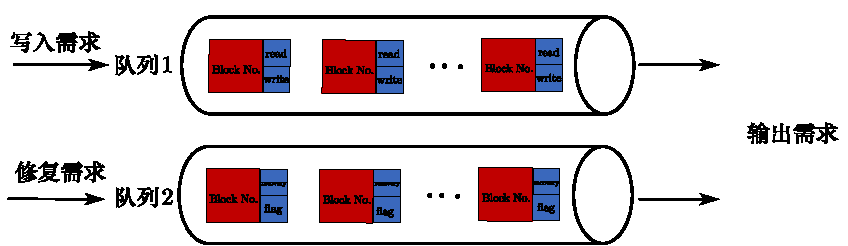
\includegraphics [scale=0.7]{figures/4.3.pdf}
	\caption{动态自适应划分冷热数据队列}
	\label{fig:4.3}
\end{figure}

用队列1来记录数据写入的信息流,其中每个块记录了块ID和缓存命中次数。
队列2存储着数据块的恢复请求,其中包含了区块ID、缓存命中次数和表示数据的编码方案。
首先将LRC$(k, l,g)$设定为整个存储系统的默认编码,两个队列在启动后会有一个默认初始化,
在自适应规则中,三个条件来触发自适应过程。 首先,对于在队列2头部插入的每个修复请求,
算法确定相关块是否需要用LRC码进行编码。 其次,对于在队列1头部插入的每个写请求,
算法确定相关的块是否需要用HH码进行编码。 最后,对于在队列2尾部删除的每个修复请求,
算法会将LRC码转换成HH码。具体的过程如算法~\ref{alg:4-1}中所示。

\begin{algorithm}[htpb]
	\begin{algorithmic}[1]
		% \newlength{\commentindent}
		\setlength{\commentindent}{.3\textwidth}
		\setlength{\algorithmicindent}{1.5em}
		\renewcommand{\algorithmiccomment}[1]{\unskip\hfill\makebox[\commentindent][l]{$\rhd$~#1}\par}
		\LetLtxMacro{\oldalgorithmic}{\algorithmic}
		\renewcommand{\algorithmic}[1][0]{
			\oldalgorithmic[#1]
			\renewcommand{\ALC@com}[1]{
				\IFnum\pdfstrcmp{##1}{default}=0\ELSE\algorithmiccomment{##1}\fi}%
		}
		\REQUIRE{Queue1,Queue2 and $\eta$}
		% \ENSURE{$\textbf{NewW}$}
        \FOR{\text{Queue2头的每个插入请求}}
        \IF{flag $\neq $ LRC and (writes/recoveries) $< \eta$}
        \STATE set flag = LRC;
        \STATE convert to LRC;
        \ENDIF
        \ENDFOR
        \FOR{\text{Queue1头的每个插入请求}}
        \IF{flag $\neq $ HH and (writes/recoveries) $\geqslant  \eta$}
        \STATE set flag = HH;
        \STATE convert to HH;
        \ENDIF
        \ENDFOR
        \FOR{\text{Queue2尾的每个弹出请求}}
        \IF{flag == LRC }
        \STATE set flag = HH;
        \STATE convert back to HH;
        \ENDIF
        \ENDFOR
		% \STATE $\textbf{NewW} = \textbf{w}$;
		% \WHILE {true}
		% \STATE R = FindMaxTimeRoad($\textbf{NewW}$);
		% \IF {type == 1}
		% \STATE S = FindNodeWithoutChunk($\textbf{NewW}$);
		% \STATE D = R.Destination;
		% \ELSE
		% \STATE S, D = R.Source, R.Destination;
		% \ENDIF
		% \STATE RIdle = GetIdleNode(R);
		% \STATE NewR = DijkstraMinTimeRoad(S, D, RIdle);
		% \STATE Update($\textbf{NewW}$, NewR);
		% \IF {FindMaxTimeRoad($\textbf{NewW}$) == R}
		% \STATE break;
		% \ENDIF
		% \ENDWHILE
		% \STATE $\textbf{return}$ $\textbf{NewW}$;
	\end{algorithmic}
	\caption{动态自适应冷热数据划分算法}
	\label{alg:4-1}
\end{algorithm}


\section{编码切换算法}

HH码和LRC码均为RS码的一种改进。在使用HH$(k,m)$码进行编码时,首先需要进行RS$(k,m)$码
的编码,在进行一系列Piggybacking框架中关于$g_i(a)$的异或运算;而在使用LRC$(k,l,g)$进行编码
时,$g$个全局冗余块需要通过执行RS$(k,g)$码的编码函数得到,而$l$个局部冗余块则需要进行异或运算得到。
另外HH$(k,m)$码中的$g_i(a)$的计算,需要将$k$个数据块分为$(m-1)$组,而LRC$(k,l,g)$中的局部冗余的
计算,则需要将$k$个数据块分为$l$组。由此,当$k_{HH}=k_{LRC}$且$m_{HH}=g_{LRC}$且$m_{HH}-1=l_{LRC}$时,
相应的HH码和LRC码可以共用一个RS码的冗余块,并且可以进行高效地切换。

记$k=k_{HH}=k_{LRC}$以及$t=m_{HH}=g_{LRC}$,则$l_{LRC}=m_{HH}-1=t-1$,系统中采用HH$(k,t)$和LRC$(k,t-1,t)$。
由于HH码会将原RS码中每两个条带视为一个条带中的两个子条带,因此此切换算法也对LRC进行类似处理,即每一个条带中都包含两个
子条带。在LRC中,一个条带中的两个子条带分别进行各自的编码;而在HH码中,其中一个条带$a$的额外冗余信息$g_i(a)$会被
异或到另一子条带$b$的冗余子块中。

从LRC$(k,t-1,t)$转换为HH$(k,t)$码时,
首先将子条带$a$中的各局部冗余子块读取并传输到对应的全局冗余块所在节点,并与该节点中子条带b的全局冗余子块进行异或运算,
之后再将各局部冗余块删除即可。详细过程如算法~\ref{alg:4-2}和图~\ref{fig:4.4}所示。

\begin{figure}[H]
	\centering
	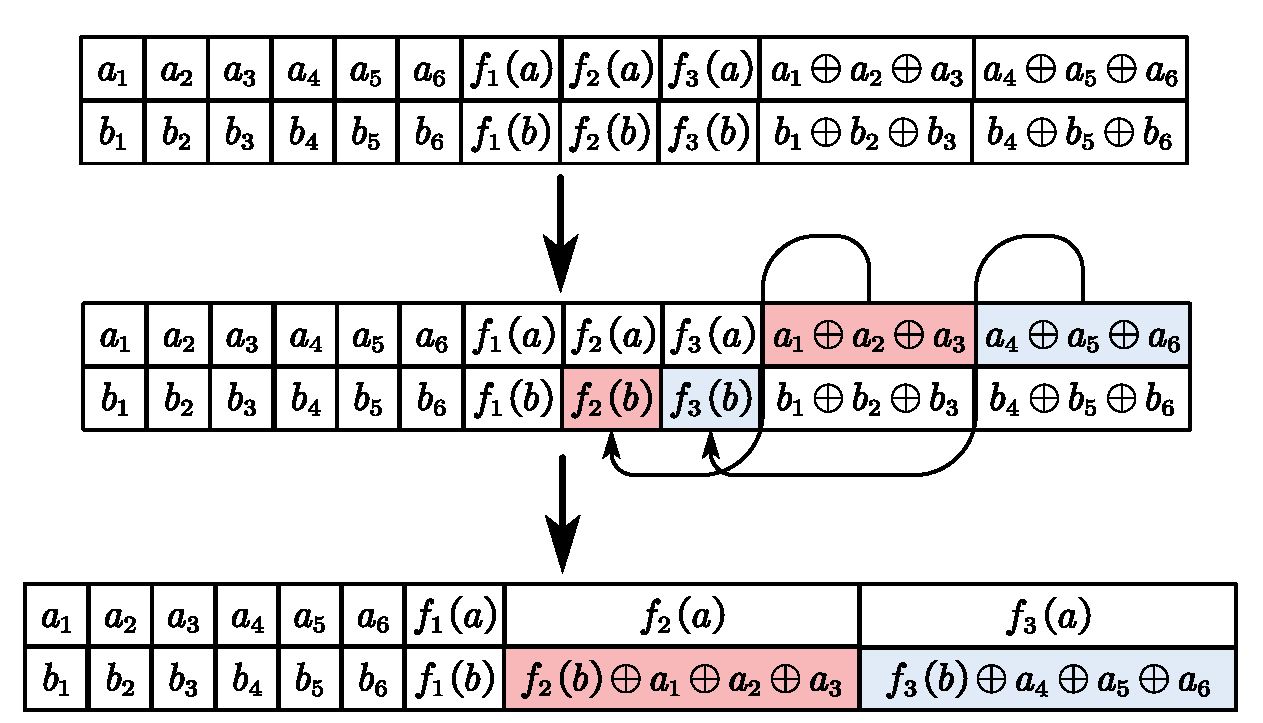
\includegraphics [scale=0.5]{figures/4.4.pdf}
	\caption{LRC$(6,2,3)\rightarrow $ HH$(6,3)$过程}
	\label{fig:4.4}
\end{figure}


\begin{algorithm}[htbp]
	\begin{algorithmic}[1]
		% \newlength{\commentindent}
		\setlength{\commentindent}{.3\textwidth}
		\setlength{\algorithmicindent}{1.5em}
		\renewcommand{\algorithmiccomment}[1]{\unskip\hfill\makebox[\commentindent][l]{$\rhd$~#1}\par}
		\LetLtxMacro{\oldalgorithmic}{\algorithmic}
		\renewcommand{\algorithmic}[1][0]{
			\oldalgorithmic[#1]
			\renewcommand{\ALC@com}[1]{
				\IFnum\pdfstrcmp{##1}{default}=0\ELSE\algorithmiccomment{##1}\fi}%
		}
		\REQUIRE{LRC中的两个子条带$a$和$b$}
		\ENSURE{HH码中的两个子条带$s_a$和$s_b$}
        \STATE $s_a.data := a.data$
        \STATE $s_b.data := b.data$
        \STATE $s_a.parity := a.global$\_$parity$
        \STATE $s_b.parity[1] := b.global$\_$parity[1]$
        \FOR{$i:=2 \, to \, t$}
        \STATE $s_b.parity[i] := b.global$\_$parity[i] \oplus a.local$\_$parity[i-1]$
        \ENDFOR
	\end{algorithmic}
	\caption{LRC$(k,t-1,t)\rightarrow $ HH$(k,t)$算法}
	\label{alg:4-2}
\end{algorithm}


从HH$(k,t)$码转换为LRC$(k,t-1,t)$时,首先计算出所有局部冗余块,
之后再将其中子条带$a$中的局部冗余子块传到对应的全局冗余块所在节点, 
并与该节点中子条带$b$的全局冗余子块进行异或运算,使得这些子条带$b$的全局冗余子块不再包含子条带$a$中
的额外冗余信息$g_i(a)$。详细过程如算法~\ref{alg:4-3}和图~\ref{fig:4.5}所示。


\begin{algorithm}[tb!]
	\begin{algorithmic}[1]
		% \newlength{\commentindent}
		\setlength{\commentindent}{.3\textwidth}
		\setlength{\algorithmicindent}{1.5em}
		\renewcommand{\algorithmiccomment}[1]{\unskip\hfill\makebox[\commentindent][l]{$\rhd$~#1}\par}
		\LetLtxMacro{\oldalgorithmic}{\algorithmic}
		\renewcommand{\algorithmic}[1][0]{
			\oldalgorithmic[#1]
			\renewcommand{\ALC@com}[1]{
				\IFnum\pdfstrcmp{##1}{default}=0\ELSE\algorithmiccomment{##1}\fi}%
		}
		\REQUIRE{HH码中的两个子条带$s_a$和$s_b$}
		\ENSURE{LRC码中的两个子条带$a$和$b$}
        \STATE $a.data := s_a.data$
        \STATE $b.data := s_b.data$
        \STATE $a.global$\_$parity := s_a.parity$
        \STATE $b.global$\_$parity[1] := s_b.parity[1]$
        \FOR{$i:=1 \, to \, t-1$}
        \STATE $a.local$\_$parity[i] := 0$
        \STATE $b.local$\_$parity[i] := 0$
            \FOR{$G_i$中的每个块$j$}
                \STATE $a.local$\_$parity[i] := a.local$\_$parity[i] \oplus a.data[j]$
                \STATE $b.local$\_$parity[i] := b.local$\_$parity[i] \oplus b.data[j]$
            \ENDFOR
        \ENDFOR
        \FOR{$i:=2 \, to \, t$}
            \STATE $b.global$\_$parity[i] := s_b.parity[i] \oplus a.local$\_$parity[i-1]$
        \ENDFOR
	\end{algorithmic}
	\caption{HH$(k,t) \rightarrow$ LRC$(k,t-1,t) $ 算法}
	\label{alg:4-3}
\end{algorithm}

\begin{figure}[htbp]
	\centering
	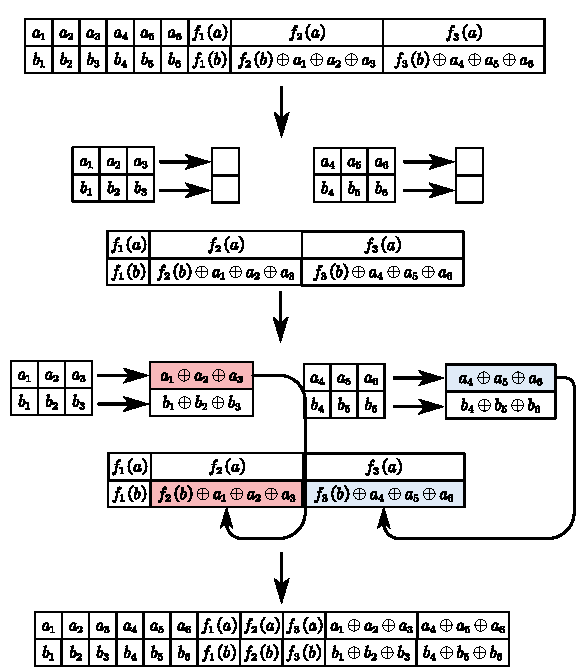
\includegraphics [scale=1.2]{figures/4.5.pdf}
	\caption{HH$(6,3) \rightarrow $ LRC$(6,2,3) $过程}
	\label{fig:4.5}
\end{figure}

\section{实验结果与分析}

\subsection{实验参数与数据集}

实验选取参数的$(k,t)=(12,4)$,即在系统中部署LRC$(12,3,4)$和HH$(12,4)$两种编码。根据这一选择,在仿真平台上
需要19个以上的节点部署,其他实验环境与第\ref{chapter:3}章一致。本文选择了四种数据集\cite{narayanan2008write}作为经典的系统运行负载如表~\ref{table:4-3}
所示,
关于每个数据集的解释如下:

\begin{itemize}
	\item \textsc{MSR-mds1},来自于媒体服务器且在四个数据集中拥有最高的读取比例;
	\item \textsc{MSR-rsrch0,MSR-rsrch2},两个数据集均通过研究项目产生,其中\textsc{MSR-rsrch0}的读取量最低,且\textsc{MSR-rsrch2}含有中等的读取量数据;
	\item \textsc{MSR-web1},通过Web/SQL服务器产生,拥有中等的读取数据量。
\end{itemize}

\begin{table}[htbp]
	% \setlength{\tabcolsep}{2.9pt}
	\centering
	\caption{数据集介绍}
	\begin{tabular}{llrlr}
		\toprule
		\textsc{数据集}     & 请求数    & 读取比    & IOPS    & 平均请求数据大小    \\[1pt]
		\midrule
		\\[-15pt]
		\textsc{MSR-mds1}                      & 1637711              & 92.88\%              & 27.29           & 113.00KB     \\
		\textsc{MSR-rsrch2}                      & 207597              & 65.69\%               & 3.54           & 8.17KB           \\
		\textsc{MSR-web1}                      & 160891              & 54.11\%               & 2.66           & 58.14KB           \\
		\textsc{MSR-rsrch0}                      & 1433655              & 9.32\%              & 23.70           & 17.86KB       \\
		\bottomrule
	\end{tabular}
	\label{table:4-3}
\end{table}



对于修复负载,在实验平台中随机初始化故障事件,然后记录故障节点的位置和时间戳。对于时间间隔的处理,计算从最后一次
发生故障的时间间隔,并通过输入的时间间隔生成满足正态分布故障概率的故障事件。对于故障位置,设置目标故障节点和
最近故障节点之间的相对距离与故障概率成反比。同样由于存储系统中98\%的故障时单节点故障\cite{xia2015tale},所以实验基于单节点故障进行。
对于\citet{wang2020adaptive}的LRC\&HH策略默认存储方式为HH码,因为他们在实验中的数据访问遵循Zipf模拟,并且没有相应的
自适应负载切换算法,所以设置为数据访问时随机切换编码策略,具体来说当数据访问产生时,随机选择是否根据当前编码策略读取数据,否则
切换为另一种编码策略从而访问数据。

此外,本文选取了四种指标作为实验结果的衡量尺度,分别为读写负载性能$\epsilon_1$,修复负载性能$\epsilon_2$,整体负载性能$\epsilon$和
临界比$\zeta$。
正如章节\ref{subsection:4.1}所分析的三种
参数的量化。具体的指标定义如下:
\begin{enumerate}
	\item 读写负载性能$\epsilon_1$,定义为读写任务中的读写操作的平均延迟,包括了计算和数据访问消耗即transmission+disk I/O;
	\item 修复负载性能$\epsilon_2$,定义为修复任务中解码操作的平均消耗,包括计算和访问消耗;
	\item 整体负载性能$\epsilon$,定义为$\epsilon=\frac{\mu_1\epsilon_1 + \mu_2\epsilon_2}{\mu_1 + \mu_2}$,这里$\mu_1$和$\mu_2$分别代表读写和修复中的请求数;
	\item 临界比$\zeta$,定义为$\zeta = \frac{1}{\epsilon \times \rho}$,表示性能优先和存储优先之间的比例,其中$\rho = \frac{k+r}{k}$。
\end{enumerate}

\subsection{读写负载性能实验结果}


在读写负载性能实验中,RS$(10,4)$在四个数据集上的的修复时间都略高于HH$(10,4)$和LRC$(12,2,3)$的方案。
其中LRC$(12,2,3)$构建的方案比HH$(10,4)$的修复速度更快一点。而利用了二者优势的LRC\&HH Random码,在重建性能
上远优于二者,这是由于在系统上冷热数据转换时,会将LRC$(k,t-1,t)$切换为HH$(k,t)$,原本的切换方式需要
传递$(k+t-1)$个块,而混合方案只需要传输$(t-1)$个子块,即$\frac{t-1}{2}$,而当$k=12$且$t=4$时,这种切换
算法只需要重新编码算法的$\frac{1}{10}$。反过来,冷数据转换为热数据时,会将HH$(k,t)$切换为LRC$(k,t-1,t)$,
若重新编码则需要传输$(t+2t-2)$个块,而切换算法只需要传输$(2k+t-1)$个子块,即$\frac{2k+t-1}{2}$块,当
$k=12$且$t=4$时,传输的数据量为原来的$\frac{1}{4}$。

在这基础上,本文算法在四个数据集上平均性能比LRC\&HH Random又有了相应的优化,平均修复时间降低了18.7\%。因为
LRC\&HH Random在存储系统的读取与修复过程中没有对数据的自适应转换做相应的优化,本文策略在读写负载上,
利用队列技术以及相应的计算分析出了负载均衡点,从而可以从图~\ref{fig:4-6}中的蓝色柱子看出,本文的策略在前三个数据集上的
优化较为明显,因为其相应的读取比很高。

\begin{figure}[htbp]
	\centering
	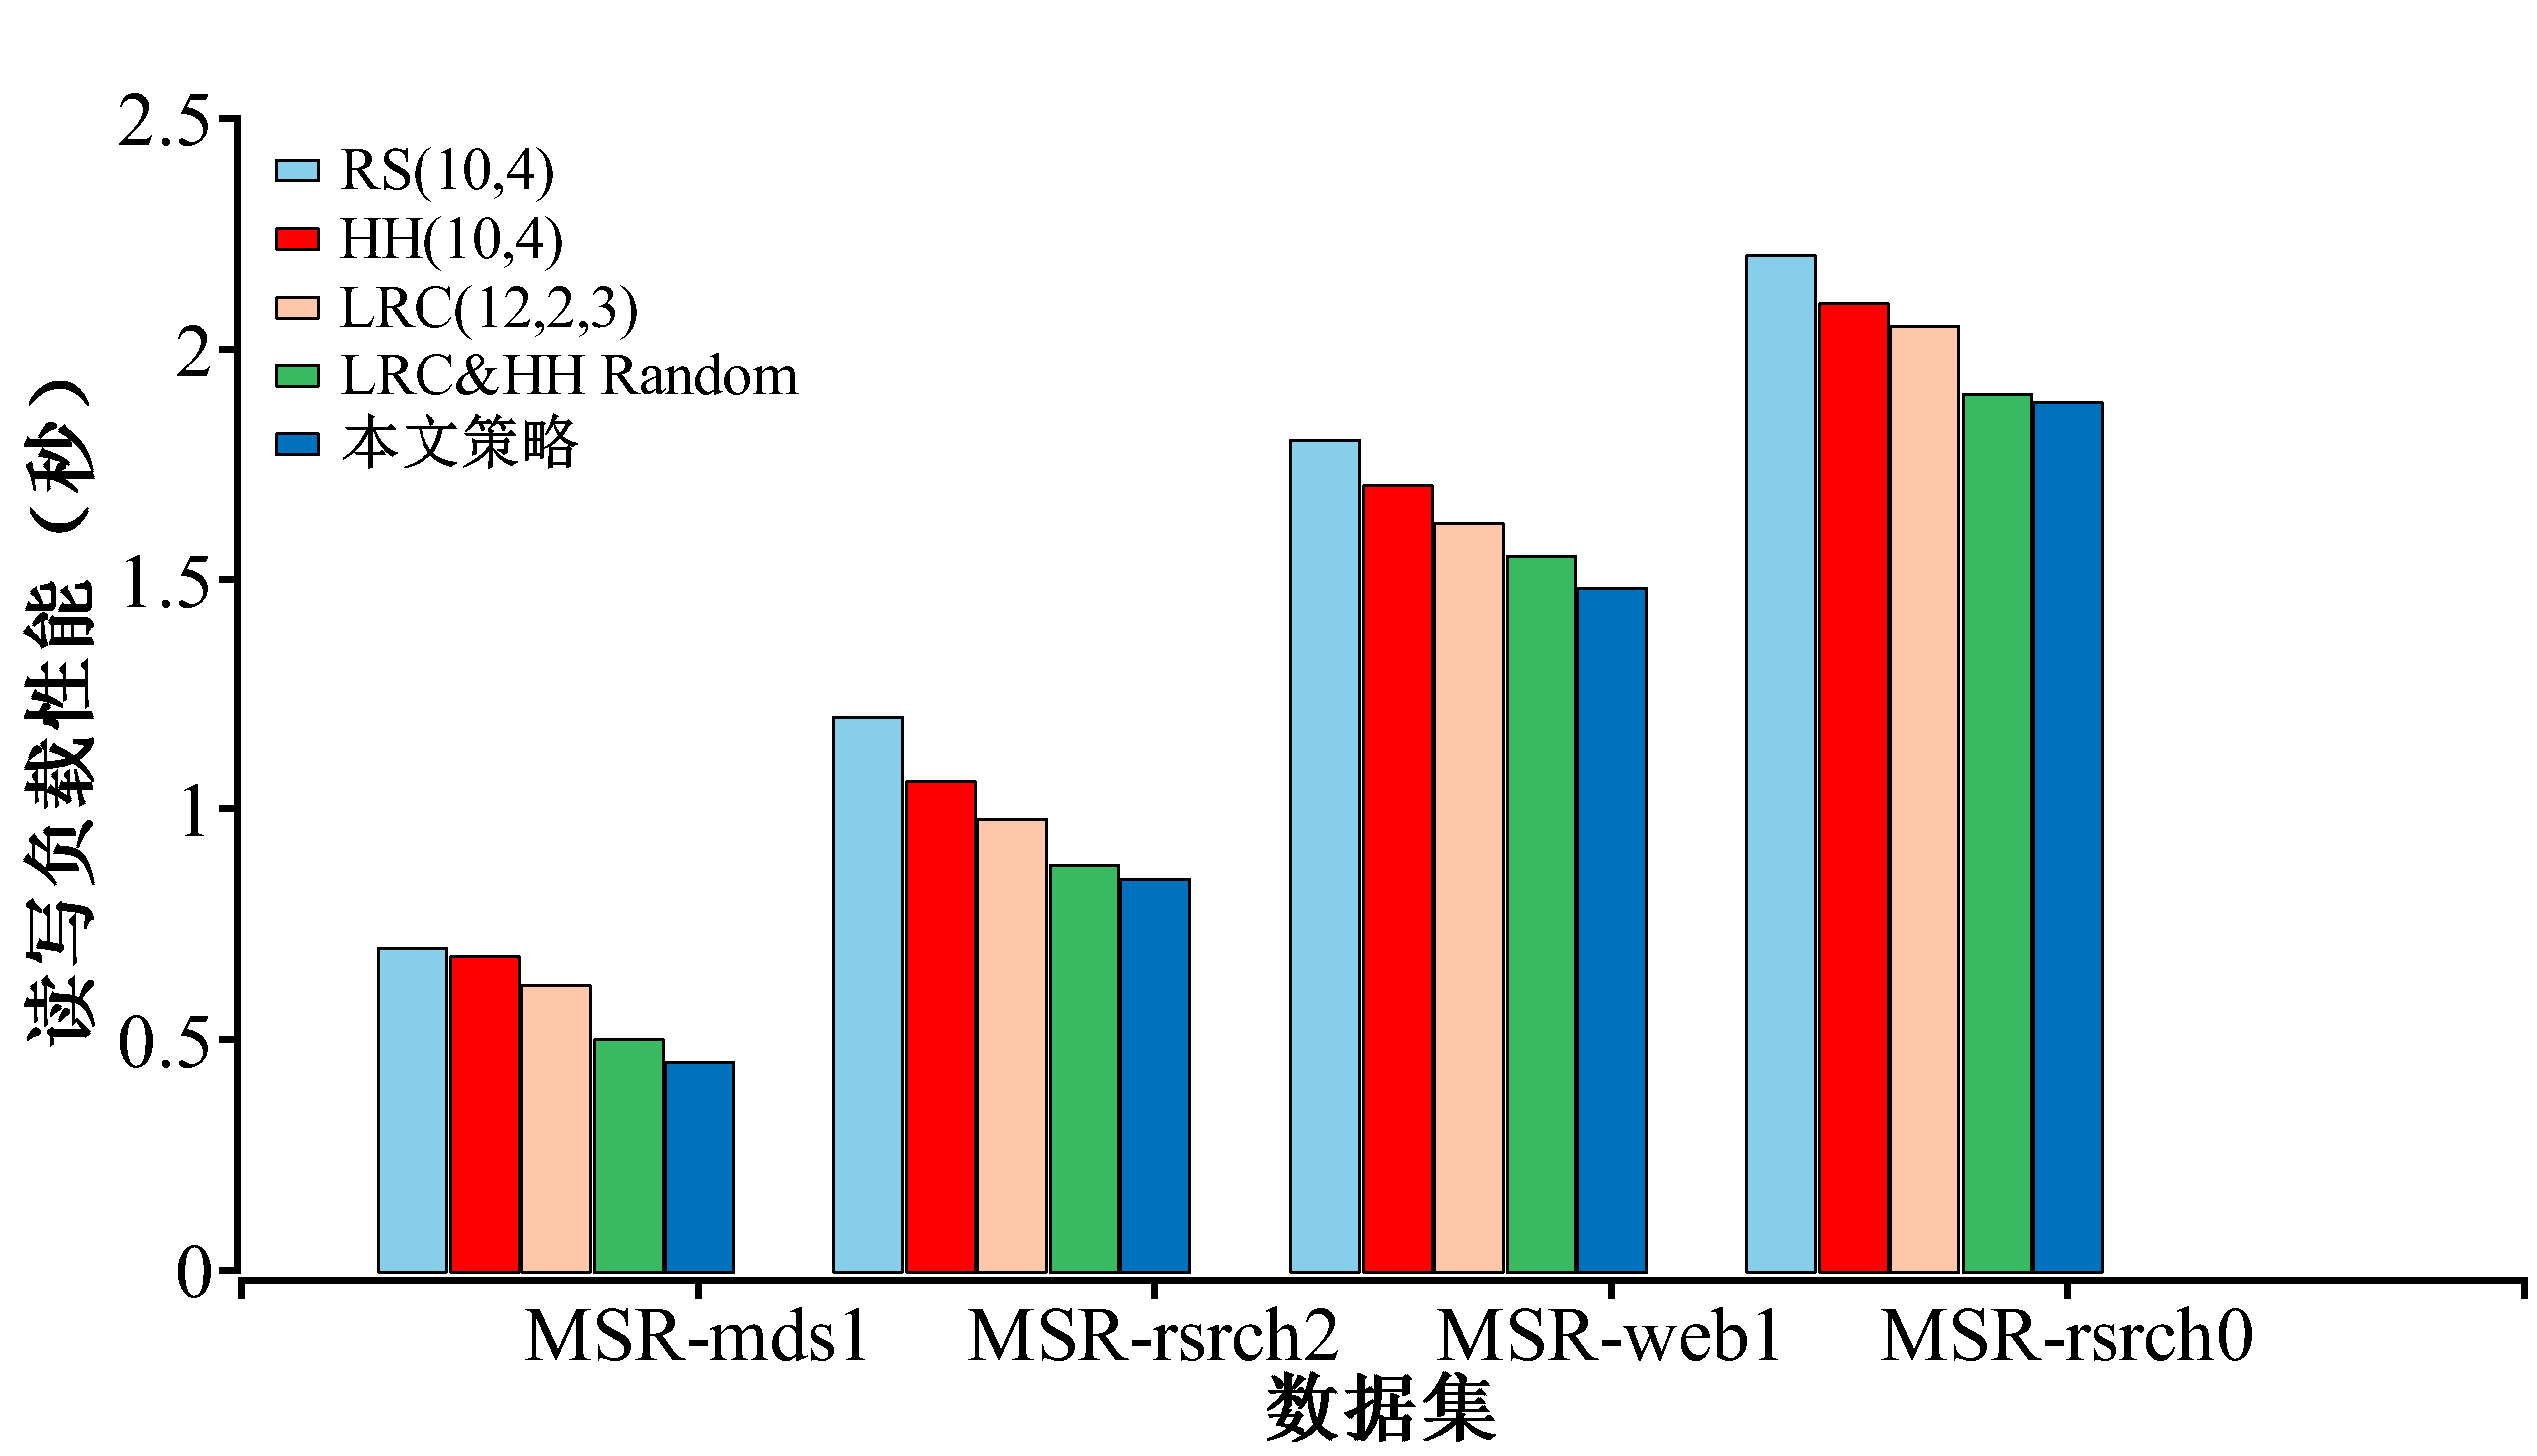
\includegraphics [scale=0.25]{figures/4-6.pdf}
	\caption{四个数据集的读写负载性能实验}
	\label{fig:4-6}
\end{figure}


\subsection{修复负载性能结果}

与读写负载实验相比,四个数据集的修复负载实验中的结果的差异化更加明显。其中,RS$(10,4)$在四个数据集上都表现出了远超于
其他方案的修复时间,主要是修复负载下,热数据的冗余更多,而RS$(10,4)$消耗了巨大的计算性能,从而拉高了修复时间。在\textsc{MSR-mds1}中,
LRC\&HH Random与本文策略的修复时间差距不大,主要是由于其具有较大的请求数、读取比以及IOPS,这样的高度集中的数据请求的情况下,
算法不能做出及时的反应。而在其他三个数据集\textsc{MSR-web1}、\textsc{MSR-rsrch2}以及\textsc{MSR-rsrch0},本文策略都用较为明显的优势,在平均性能上降低了9.4\%的修复时间。

\begin{figure}[htbp]
	\centering
	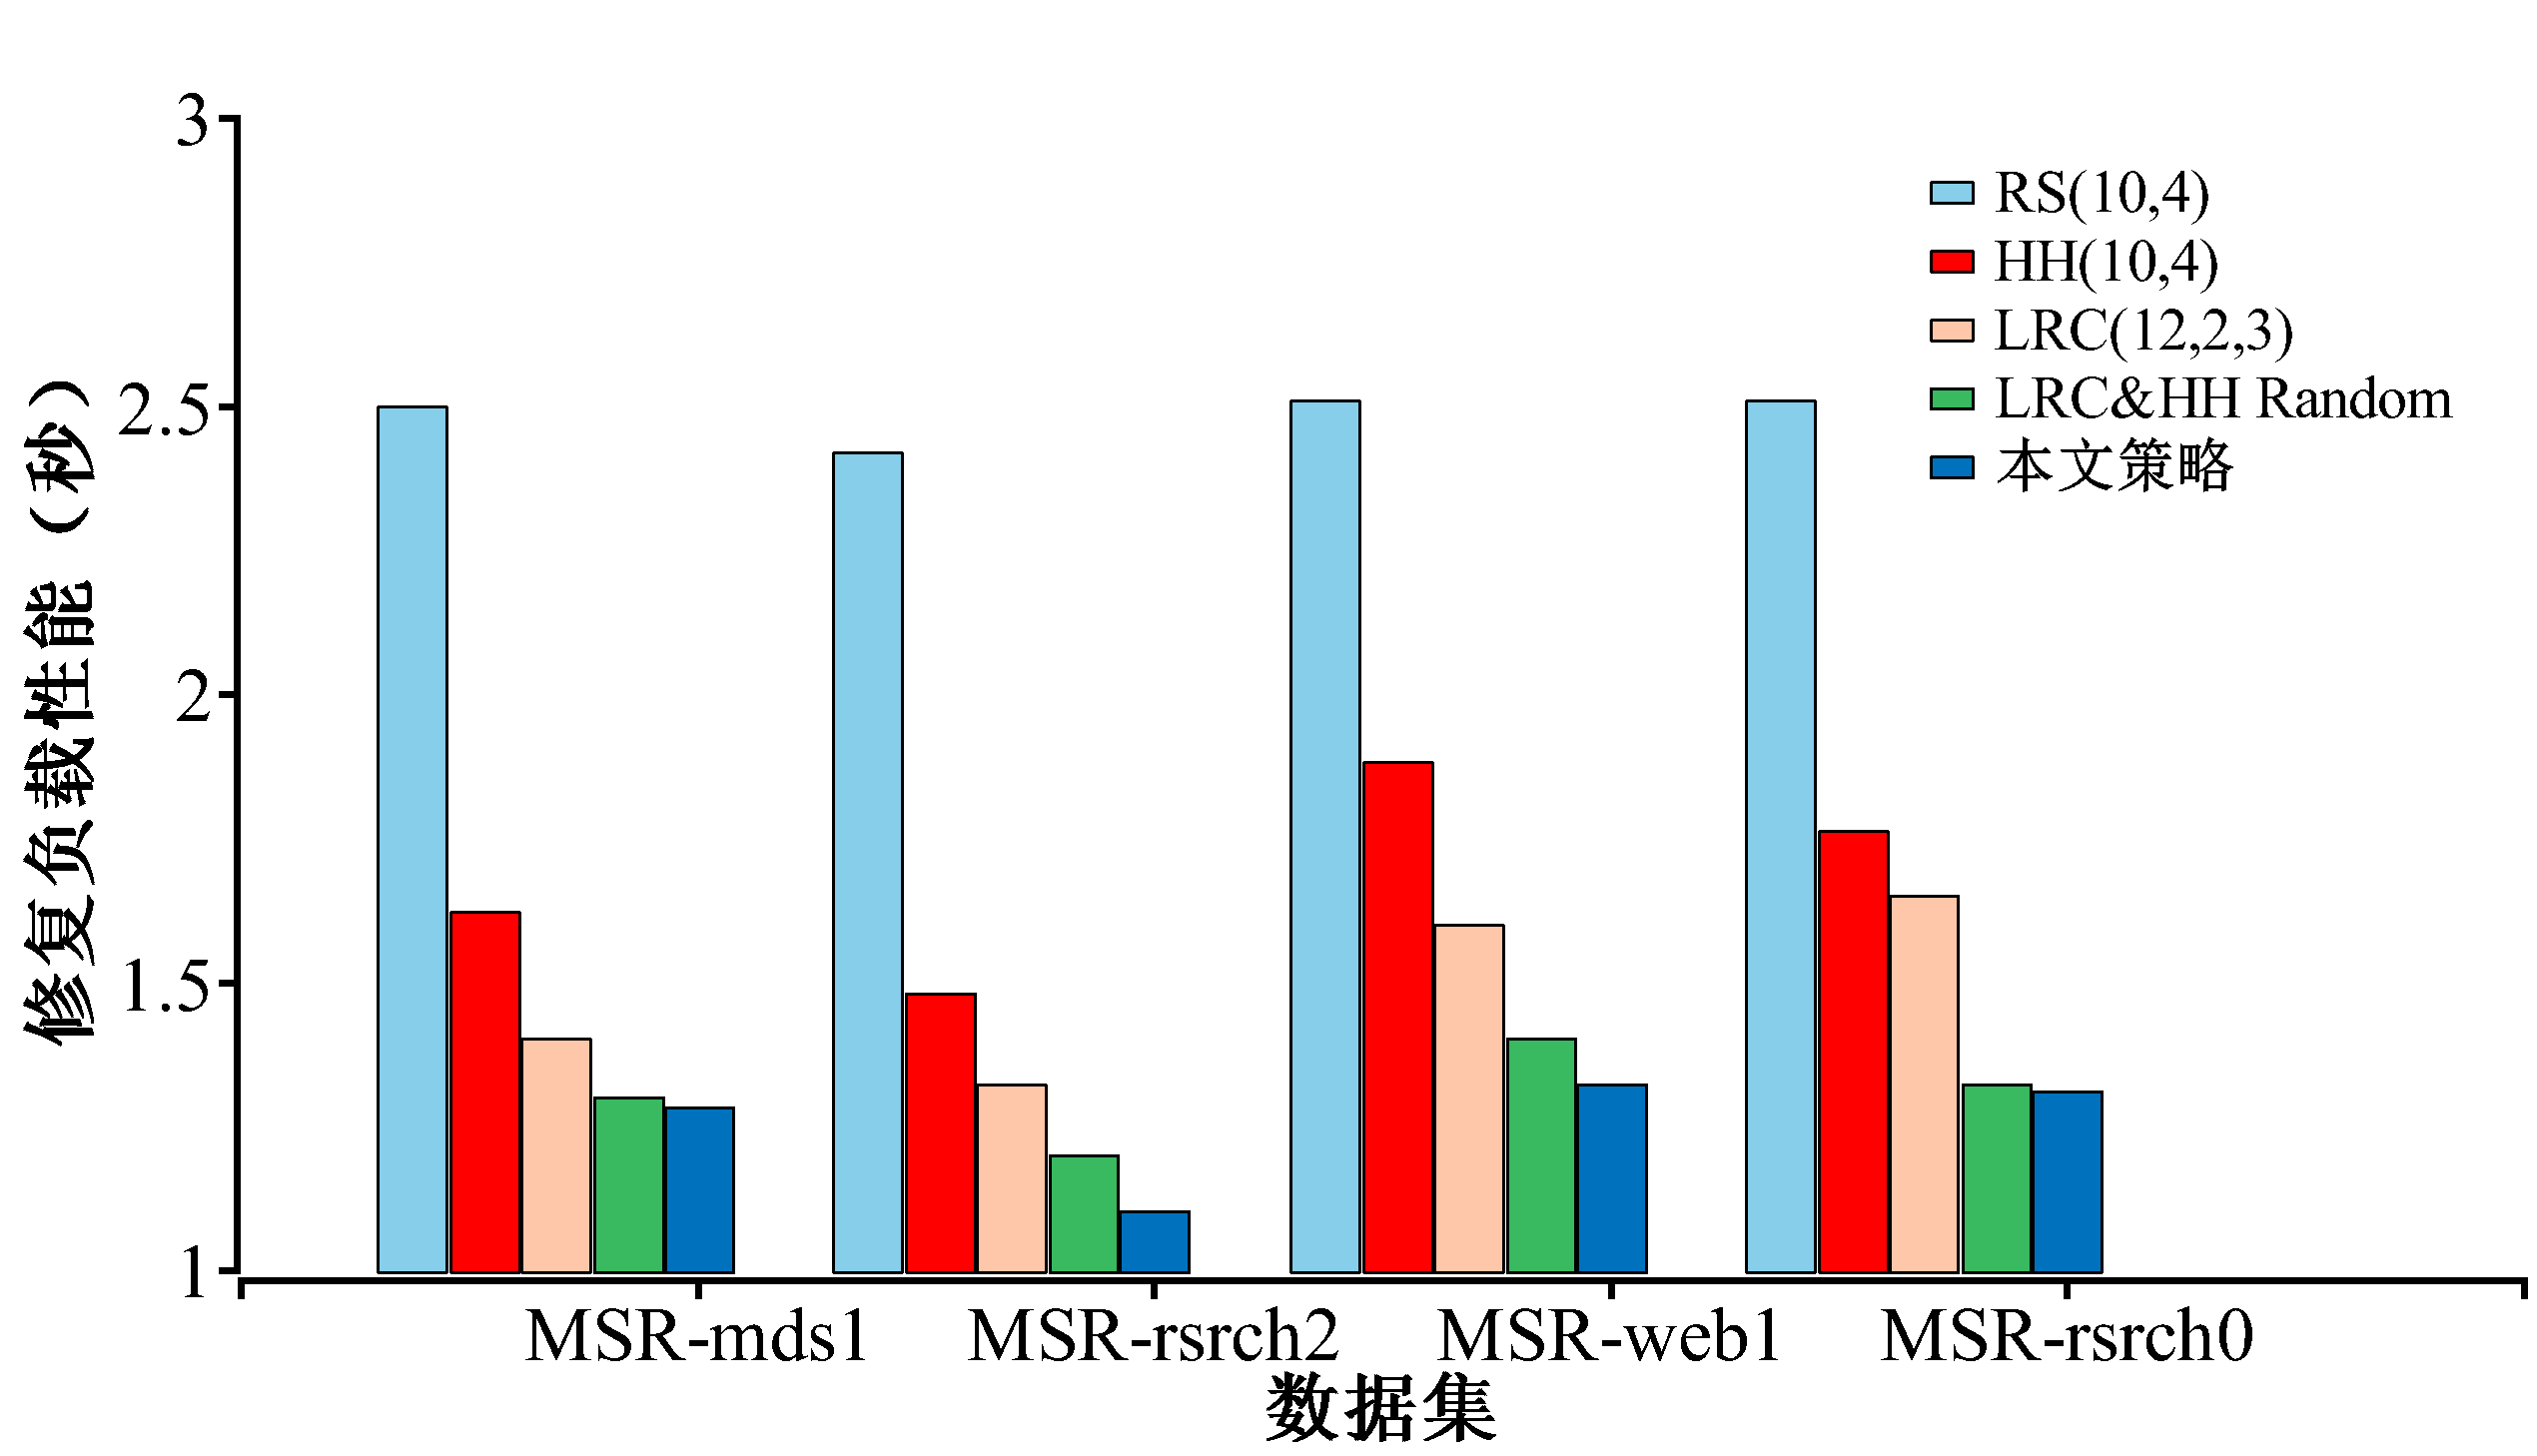
\includegraphics [scale=0.25]{figures/4-7.pdf}
	\caption{四个数据集的修复负载性能实验}
	\label{fig:4-7}
\end{figure}



\subsection{整体负载性能实验结果}


在整体性能实验中,即将读写和修复任务均匀地分摊到系统事件中,从而观察各个策略的修复性能。从图~\ref{fig:4-8}可以看出,在
读写和修复交叉的任务中,RS$(10,4)$在不同数据集上的修复性能有所上升。此外HH$(10,4)$和LRC$(12,2,3)$在不同数据集上的差异
很小,在\textsc{MSR-rsrch0}上,HH$(10,4)$的修复时间最高,且LRC\&HH Random的平均性能还是会优于其他的单一纠删码,因为
在整体负载情况下,切换任务时有发生。但是由于切换时机的随机性,本文策略在基于实时的冷热数据优化算法以及自适应策略的帮助下,
在大部分情况下依然优于随机切换的方式,平均性能上降低了6.8\%的修复时间。此外,在计算效率方面,这两种策略都是进行XOR运算,
且涉及范围相对整一组数据较小,这对比重新编码算法需要整份数据进行的伽罗瓦运算也有了明显的优化,大大提升了计算效率。


\begin{figure}[htbp]
	\centering
	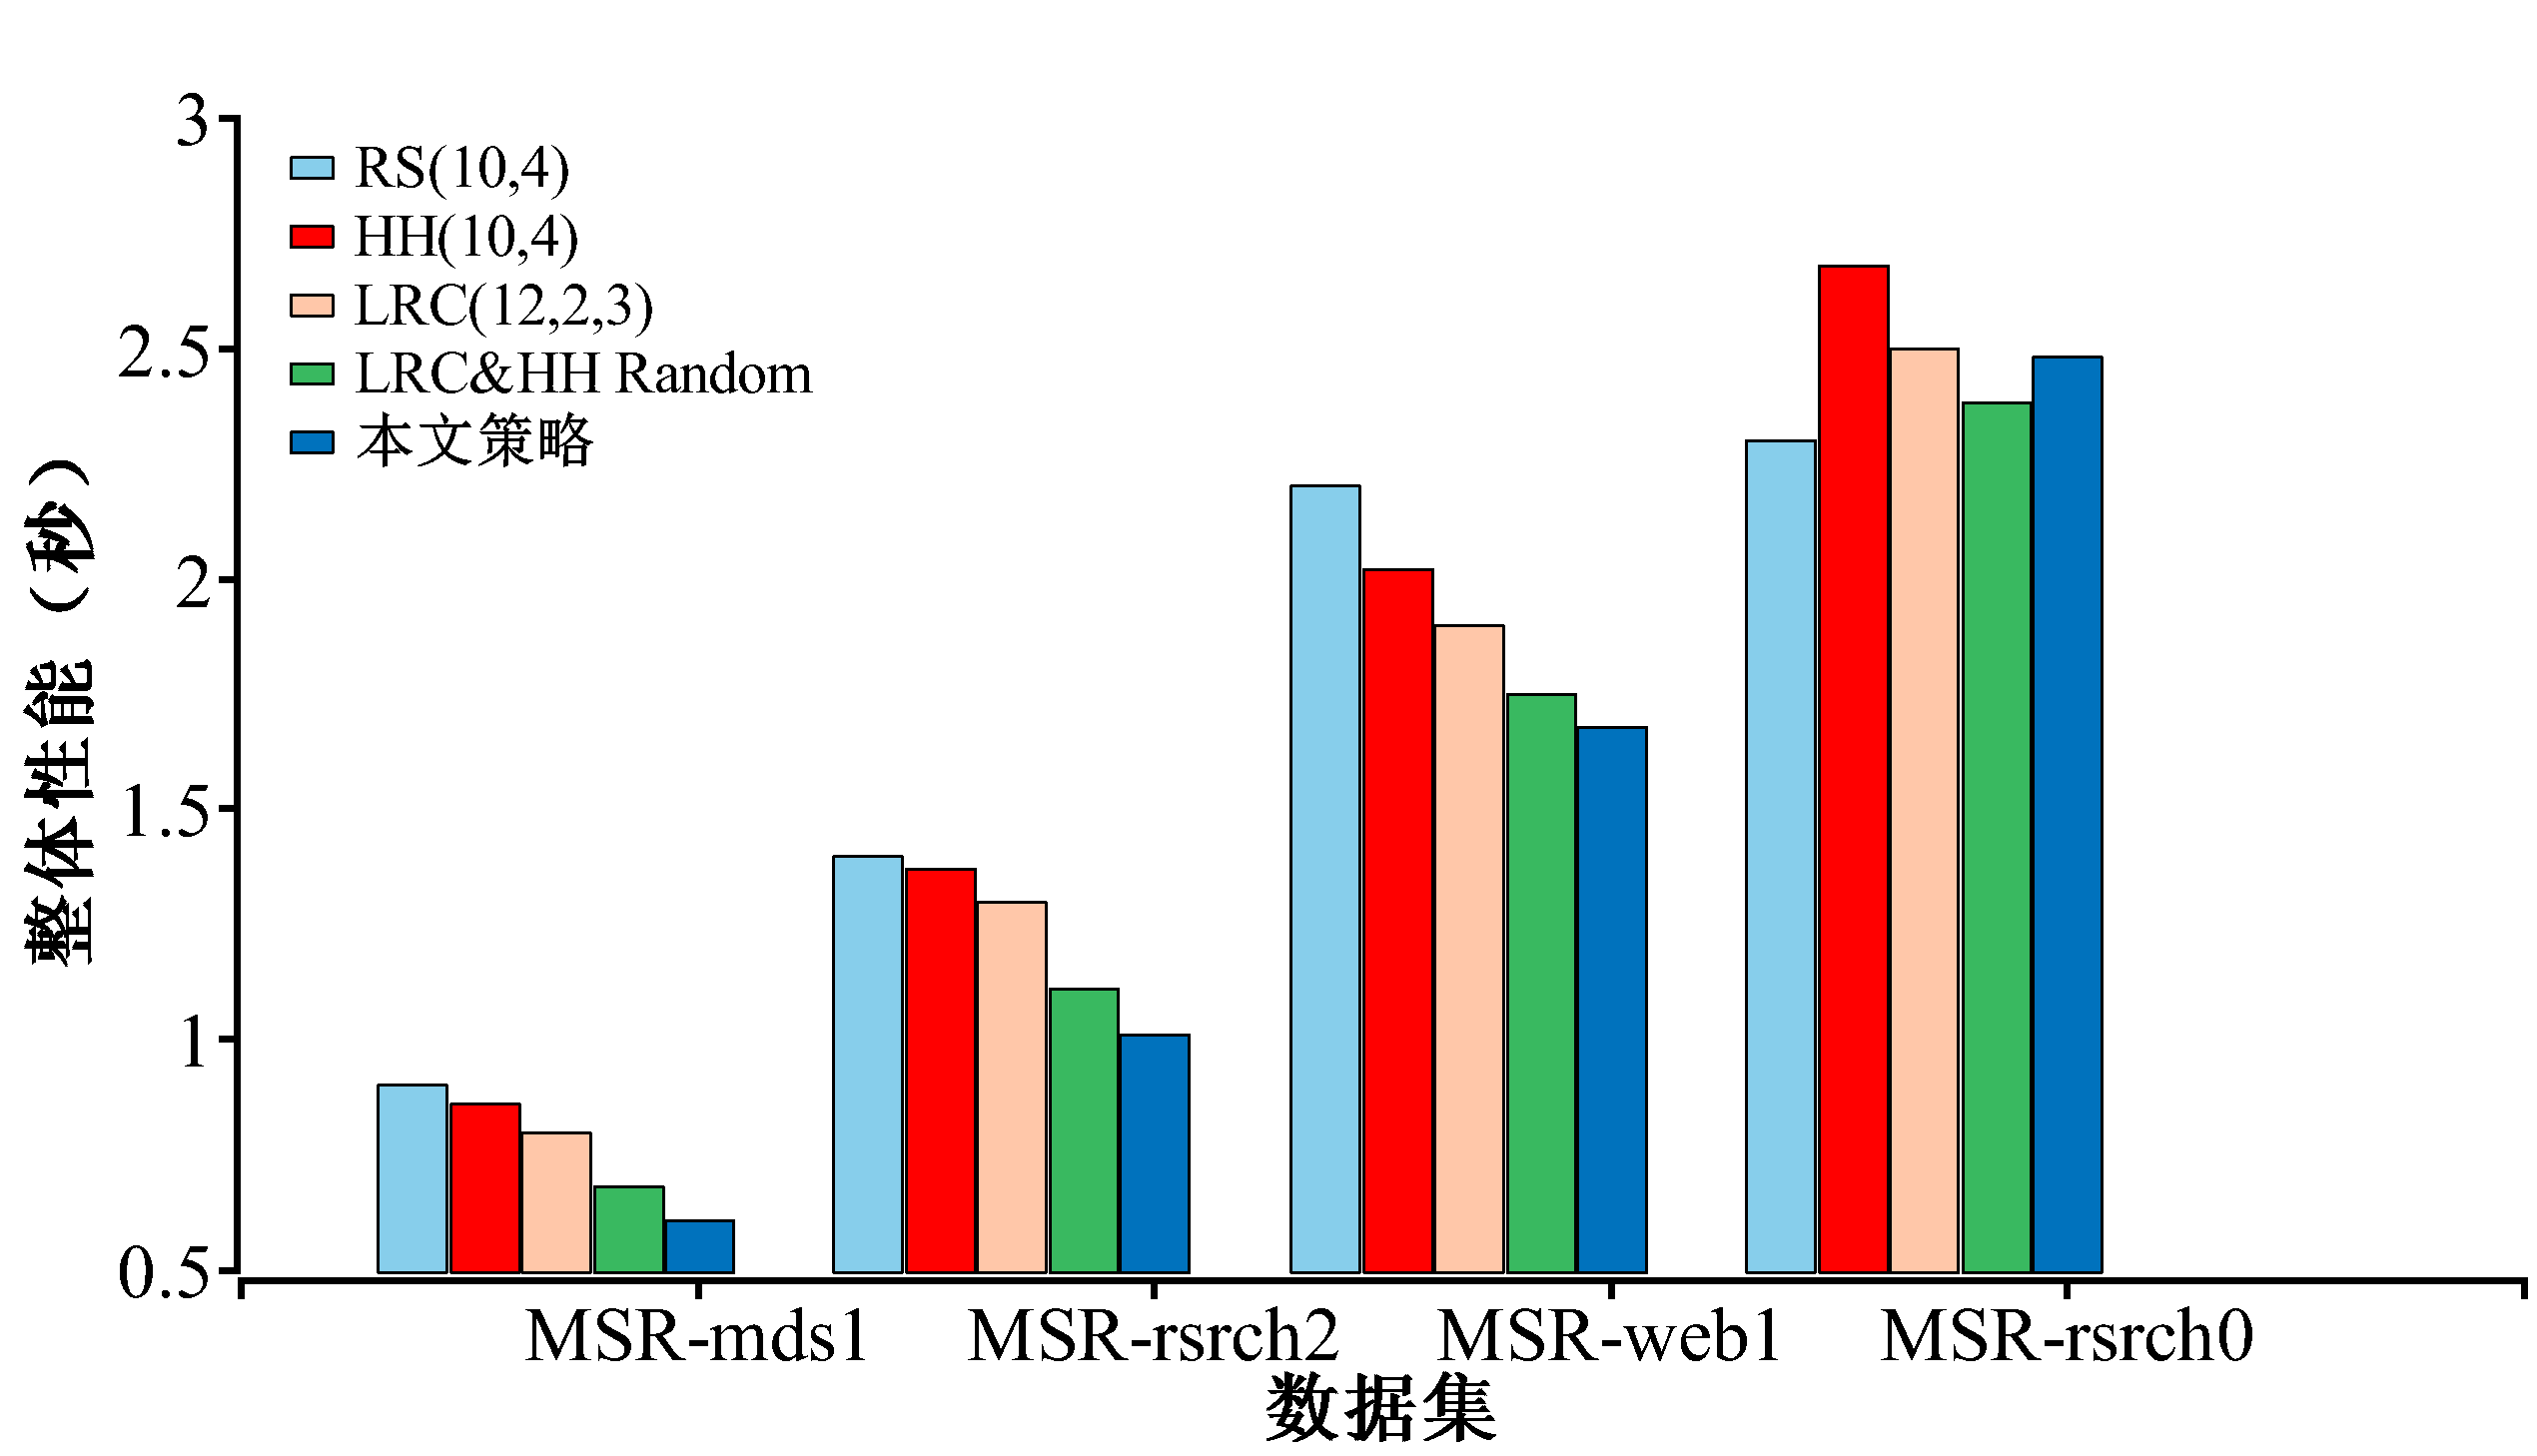
\includegraphics [scale=0.2]{figures/4-8.pdf}
	\caption{四个数据集的整体负载性能实验}
	\label{fig:4-8}
\end{figure}

\subsection{临界比实验结果}

临界比是一种衡量修复消耗的参数,数值越低则代表具有相应更低的修复消耗,修复性能更加优越。从图~\ref{fig:4-9}可以看出,
LRC$(12,2,3)$在四个数据集上都有着较高的临界比,意味着更加低的修复性能,与之相类似的是HH$(10,4)$,在前两个数据集上的
数值基本下基本相同。在平均性能上,本文策略的临界比相较于LRC\&HH Random低5.8\%。

\begin{figure}[htbp]
	\centering
	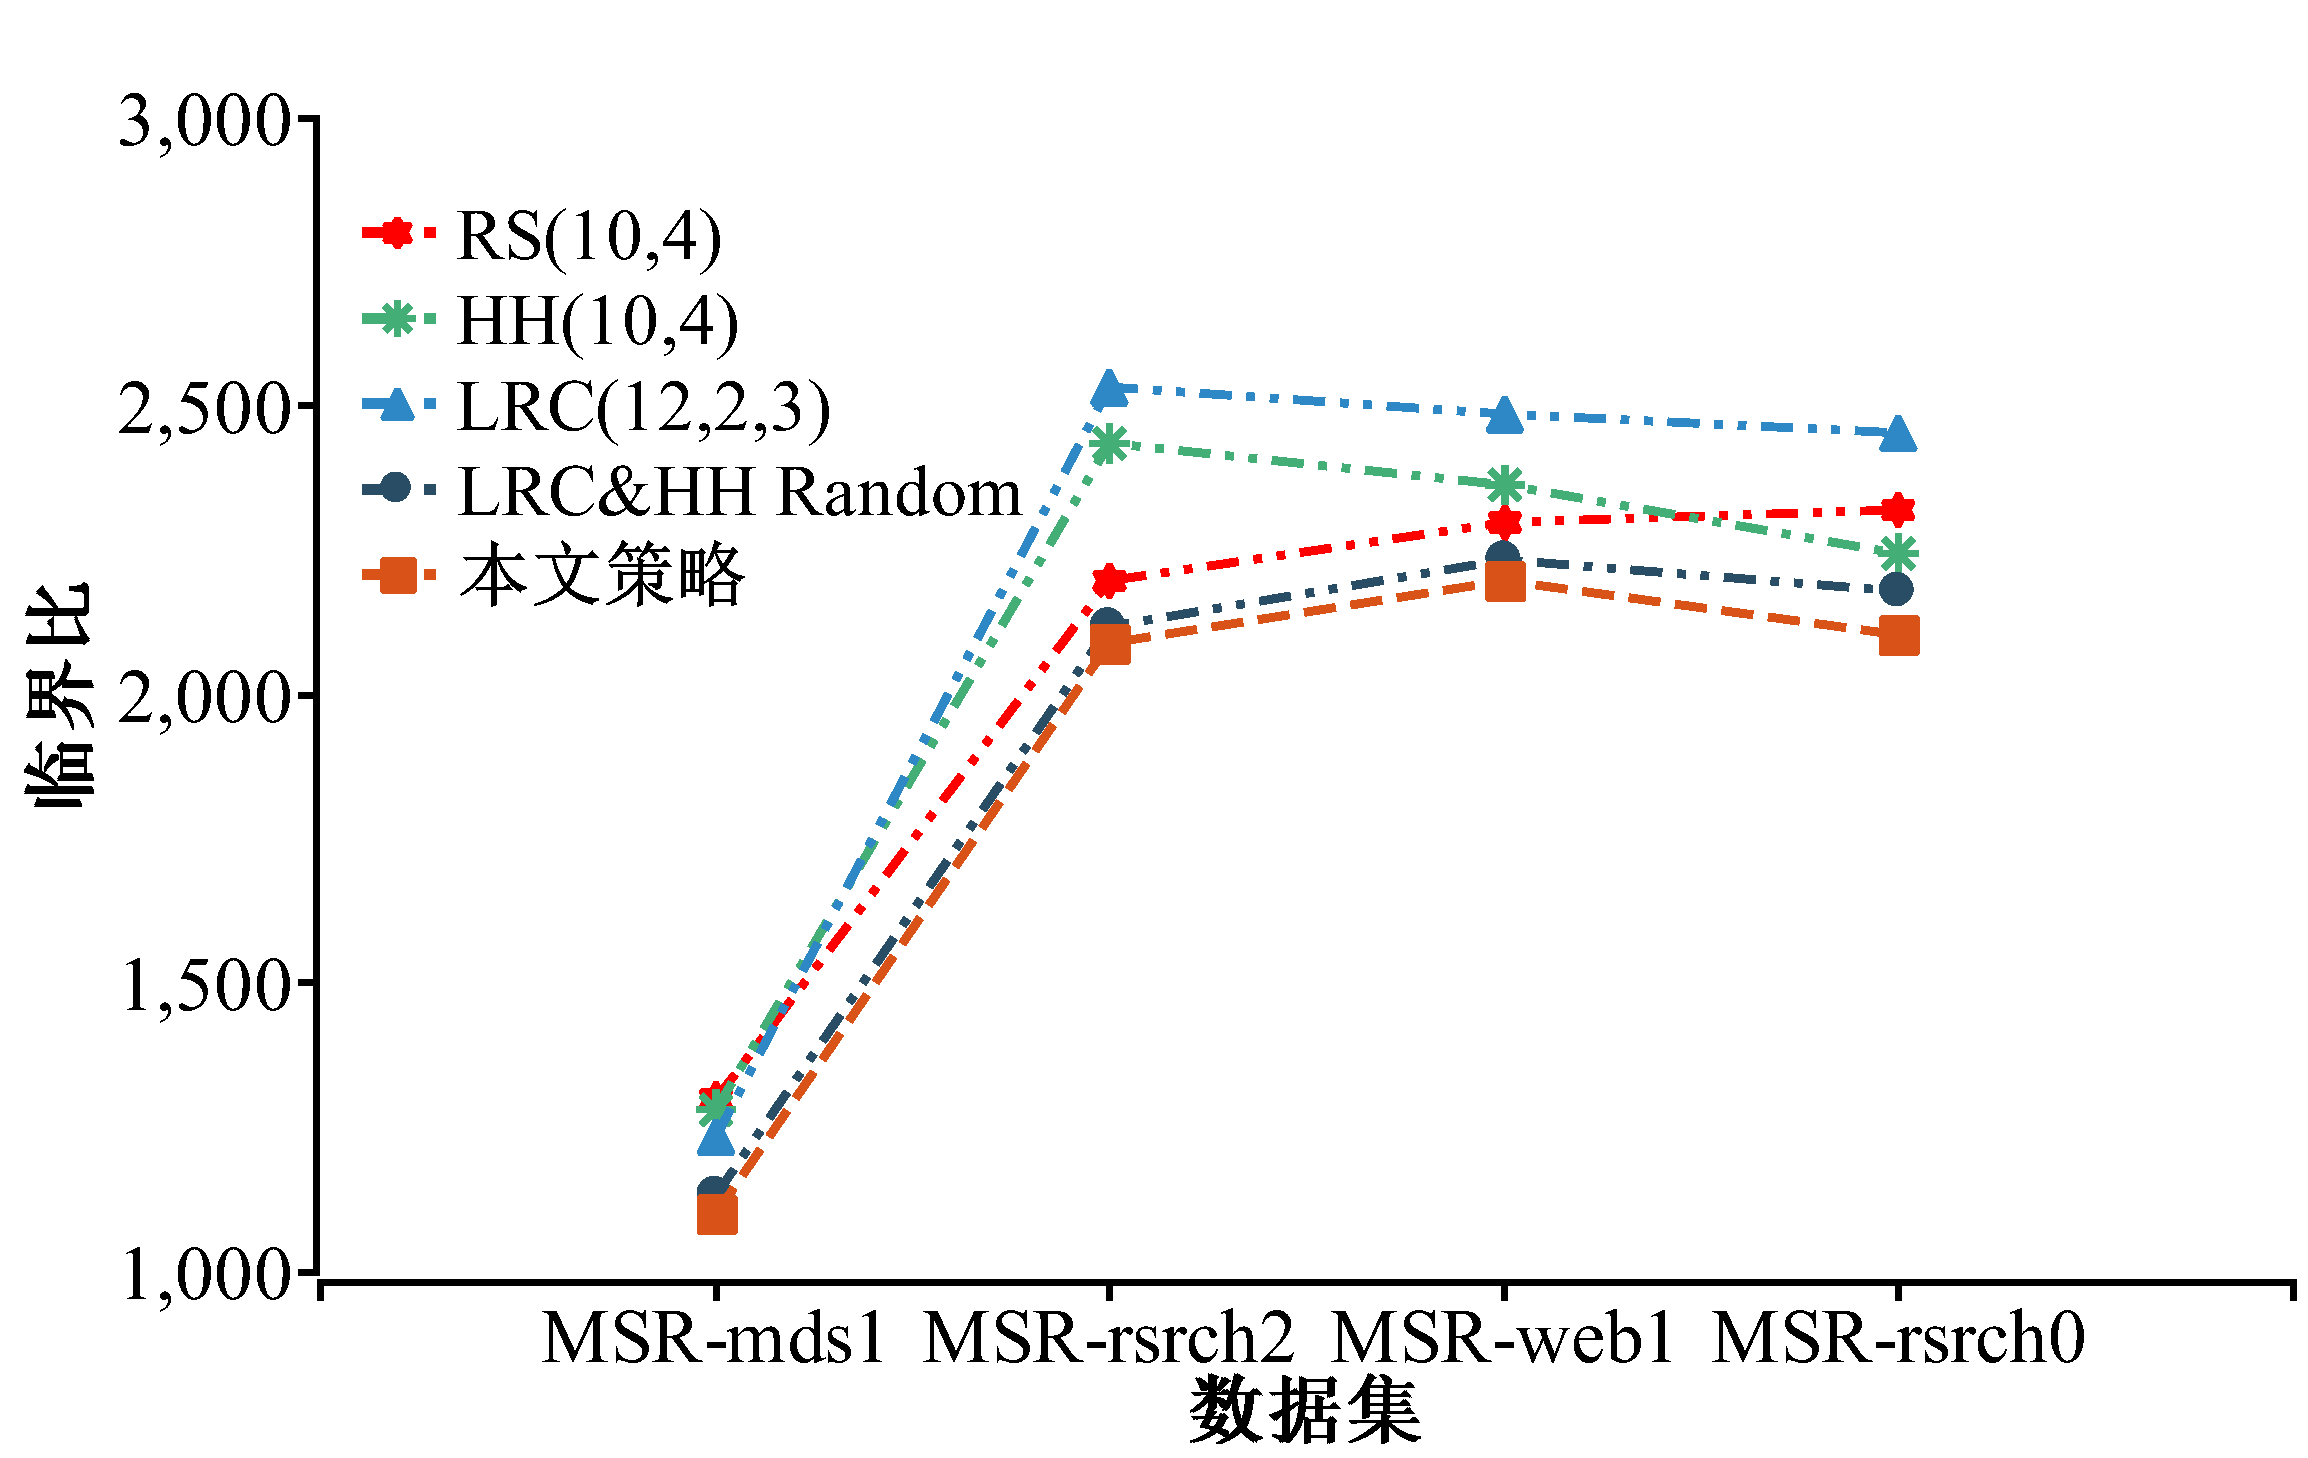
\includegraphics [scale=0.25]{figures/4-9.pdf}
	\caption{四个数据集的临界比实验}
	\label{fig:4-9}
\end{figure}


\section{本章小结}
针对在传统的存储系统中大多只采用一种纠删码进行数据的处理和存储,难以在保持低存储空间消耗的情况下降低退化读的延迟时间问题。
本文在前文预先修复的单一纠删码的基础上,进一步推进了纠删码修复技术的
应用,提出了一种可感知数据热度的负载动态自适应
的混合纠删码(LRC\&HH)数据修复方案。静态地将数
据分为六类,分别根据读写负载平衡和修复负载,根据数学计算提出相应的负载均衡策略,使用
LRU 算法来为冷热数据划分定制自适应选择算法。选取四个数据集,分别对读写负载,修复负载,
整体负载和临界比进行了对比实验,实验结果表明,
本文策略相较于LRC\&HH Random降低了6.8\%$\sim$18.7\%的修复时间。